\documentclass[../main.tex]{subfiles}

\begin{document}

\begin{definition}
A $p$ dimension \textbf{foliation}\index{Foliation} of an $n$ dimensional manifold $M$ is decomposition of $M$ into disjoint connected submanifolds $\displaystyle M=\bigsqcup_{\alpha\in A} N_\alpha$ such that for each point $p\in M$, there is a neighborhood of $p$ and a local chart $(x^1,\cdots,x^n)$ such that each $N_\alpha\cap M$ is given by $x^{p+1}=\mathrm{const},\cdots,x^n=\mathrm{const}$
\begin{center}
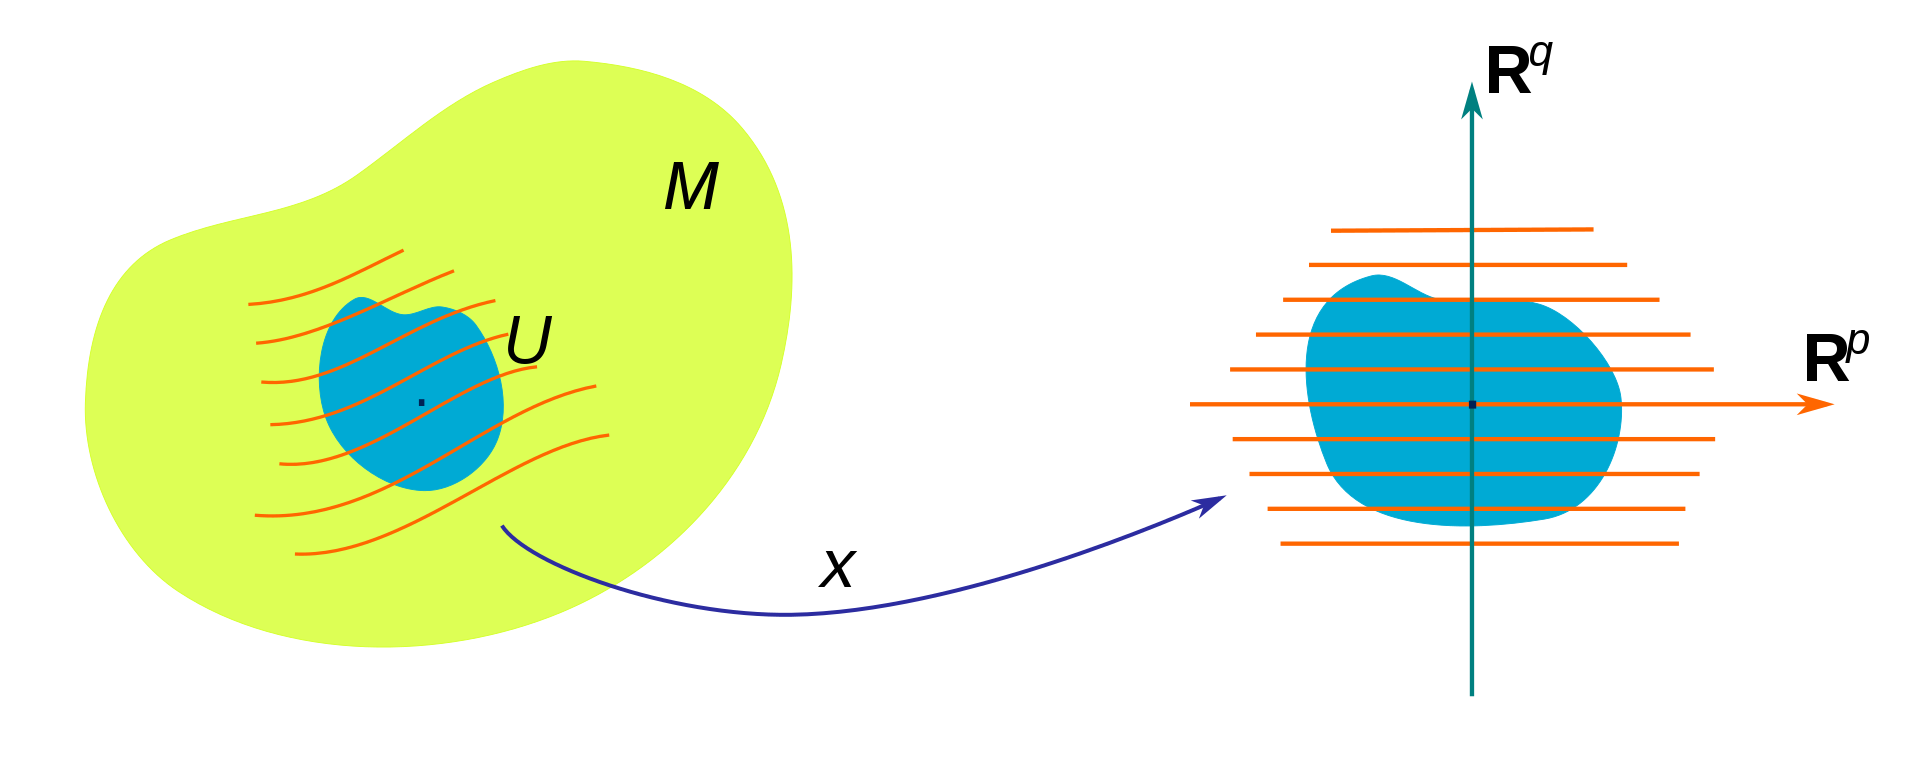
\includegraphics[scale=0.1]{Pictures/Foliation.png}
\end{center}
\end{definition}

\begin{definition}
An \textbf{integral submanifold}\index{Integral submanifold} $N\subseteq M$ is a submanifold such that locally $TN=\mathrm{Span}(X_1,\cdots,X_n)$ where $X_i$ is a local basis, $1$-dimensional integral submanifolds are just \textbf{integral curves}\index{Integral curve}
\end{definition}

\begin{definition}
Suppose $M$ is a smooth manifold of dimension $m$, an $n$-dimensional \textbf{distribution}\index{Distribution(Differential geometry)} over $M$ is
\[\Delta=\bigsqcup_{p}\Delta_p\subseteq TM, \Delta_p\leq T_pM, \dim\Delta_p=n\]
Which is locally spanned by a local basis $X_1,\cdots,X_n$
\end{definition}

\begin{remark}
We can also define distributions on vector bundles
\end{remark}

\begin{definition}
$\Delta$ is \textbf{involutive}\index{Involutive distribution} if $[\Delta,\Delta]\subseteq\Delta$, $\Delta$ is \textbf{integrable}\index{Integrable distribution} if for any point $p\in M$, there exists a integral submanifold $N\ni p$ such that $T_pN=\Delta_p$
\end{definition}

\begin{lemma}\label{Involutive distribution is integrable}
If distribution $\Delta$ is integrable, then it is involutive
\end{lemma}

\begin{proof}
Since $\Delta$ is integrable, for any $p\in M$, there is a integral submanifold $N\ni p$ such that $i_*:T_pN\hookrightarrow T_pM$ is injective with $i_*(T_pN)=\Delta_p$. Suppose $X,Y\in\Delta_p$, by the naturality of Lie bracket, $[X,Y]=i_*[i_*^{-1}X,i_*^{-1}Y]\in\Delta_p$
\end{proof}

\begin{example}
Consider $D=\langle V,W\rangle$ is a two dimensional distribution over $\mathbb R^3$, where $V=\dfrac{\partial}{\partial x}+y\dfrac{\partial}{\partial z}$, $W=\dfrac{\partial}{\partial y}$, but $[X,Y]=-\dfrac{\partial}{\partial z}\notin D$, thus $D$ is not involutive, by Lemma \ref{Involutive distribution is integrable}, $D$ is not integrable
\end{example}

\begin{definition}
An $n$-dimensional distribution $D$ over a $m$-dimensional smooth manifold $M$ is \textbf{completely integrable}\index{Completely integrable distribution} if for each point $p\in M$, there is a local coordinate chart $(U,\phi)$, such that $\phi:U\to\mathbb R^n\times\mathbb R^{m-n}$ with $\phi(D)\subseteq\mathbb R^n$
\begin{center}
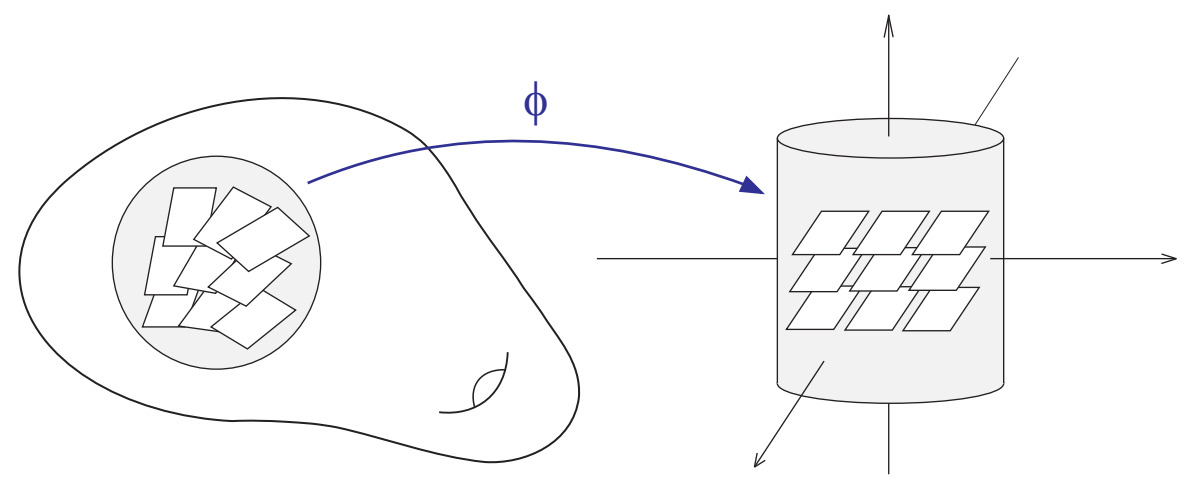
\includegraphics[scale=0.2]{Pictures/Completely_integrable.png}
\end{center}
\end{definition}

\begin{lemma}\label{Lemma for Frobenius theorem}
Suppose $M$ is an $m$ dimensional manifold, $D$ is an $n$-dimensional distribution around $p\in M$, $(U,x)$ with $x(p)=0$ is a local coordinate chart, then $D$ has a local basis $X_1,\cdots,X_n$ around $p$ such that such that
\[X_i=\frac{\partial}{\partial x^i}+\sum_{j=n+1}^ma^j_i\frac{\partial}{\partial x^j}\]
Or in matrix form
\[\begin{pmatrix}
X_1 \\
\vdots \\
X_n
\end{pmatrix}=\begin{pmatrix}
1&\cdots&0&a^{n+1}_1&\cdots&a^m_1 \\
\vdots&\ddots&\vdots&\vdots&\ddots&\vdots \\
0&\cdots&1&a^{n+1}_n&\cdots&a^m_n \\
\end{pmatrix}\begin{pmatrix}
\frac{\partial}{\partial x^1} \\
\vdots \\
\frac{\partial}{\partial x^m}
\end{pmatrix}\]
\end{lemma}

\begin{proof}
First pick a local basis $Y_1,\cdots,Y_n$ around $p$, then we have $\displaystyle Y_i=\sum_{j=1}^mb^j_i\frac{\partial}{\partial x^j}$, or in matrix form
\[\begin{pmatrix}
Y_1 \\
\vdots \\
Y_n
\end{pmatrix}=\begin{pmatrix}
b^{1}_1&\cdots&b^m_1 \\
\vdots&\ddots&\vdots \\
b^{1}_n&\cdots&b^m_n \\
\end{pmatrix}\begin{pmatrix}
\frac{\partial}{\partial x^1} \\
\vdots \\
\frac{\partial}{\partial x^m}
\end{pmatrix}\]
Since $Y_i$'s are linearly independent, $B$ is of full rank, reorder if needed, we can assume
\[\widetilde B=\begin{pmatrix}
b^{1}_1&\cdots&b^n_1 \\
\vdots&\ddots&\vdots \\
b^{1}_n&\cdots&b^n_n \\
\end{pmatrix}\]
Is invertible, we can thus define $\begin{pmatrix}
I& A
\end{pmatrix}=\widetilde B^{-1}B$, $X=\widetilde B^{-1}Y$
\end{proof}

\begin{corollary}\label{Involutive distribution ensure the existence of commuting basis}
Suppose $M$ is an $m$ dimensional manifold, $D$ is an $n$-dimensional involutive distribution around $p\in M$, then $D$ has a local basis $X_1,\cdots,X_n$ around $p$ such that such that $[X_i,X_j]=0$. In other words, we can choose a local commuting basis
\end{corollary}

\begin{proof}
Suppose $(U,x)$ with $x(p)=0$ is a local coordinate chart, by Lemma \ref{Lemma for Frobenius theorem}, $D$ has a local basis $X_1,\cdots,X_n$ around $p$ such that such that
\[X_i=\frac{\partial}{\partial x^i}+\sum_{j=n+1}^ma^j_i\frac{\partial}{\partial x^j}\]
Then
\begin{align*}
[X_i,X_j]&=\left[\frac{\partial}{\partial x^i}+\sum_{k=n+1}^ma^k_i\frac{\partial}{\partial x^k},\frac{\partial}{\partial x^j}+\sum_{l=n+1}^ma^l_j\frac{\partial}{\partial x^l}\right] \\
&=\sum_{k=n+1}^m\left[a^k_i\frac{\partial}{\partial x^k},\frac{\partial}{\partial x^j}\right]+\sum_{l=n+1}^m\left[\frac{\partial}{\partial x^i},a^l_j\frac{\partial}{\partial x^l}\right]+\sum_{k,l=n+1}^m\left[a^k_i\frac{\partial}{\partial x^k},a^l_j\frac{\partial}{\partial x^l}\right] \\
&=\sum_{k=n+1}^m\frac{\partial a^k_i}{\partial x^j}\frac{\partial}{\partial x^k}+\sum_{l=n+1}^m\frac{\partial a^l_j}{\partial x^i}\frac{\partial}{\partial x^l}+\sum_{k,l=n+1}^m\left(a^k_i\frac{\partial a^l_j}{\partial x^k}\frac{\partial}{\partial x^l}-a^l_j\frac{\partial a^k_i}{\partial x^l}\frac{\partial}{\partial x^k}\right)
\end{align*}
Is in the span of $\displaystyle\left\{\frac{\partial}{\partial x^{n+1}},\cdots,\frac{\partial}{\partial x^m}\right\}$, on the other hand, since $D$ is involutive, $[X_i,X_j]$ is also in the span of $\{X_1,\cdots,X_n\}$, thus $[X_i,X_j]=0$
\end{proof}

\begin{theorem}[Frobenius theorem]\label{Frobenius theorem}\index{Frobenius theorem}
If distribution $D$ is involutive, then it is completely integrable, alternatively, we could say that maximal integrable submanifolds form a foliation of $M$
\end{theorem}

\begin{remark}
Frobenius theorem can be thought of as a generalization of the existence theorem in ODE
\end{remark}

\begin{proof}
It suffices to show that for any $p\in M$, there is a local coordinate chart $x:U\to\mathbb R^m$ such that locally $D$ is spanned by $\left\{\dfrac{\partial}{\partial x^1},\cdots,\dfrac{\partial}{\partial x^n}\right\}$, then integrable submanifolds are just $\{x^1,\cdots,x^{n-1}\text{ are constants}\}$, we prove this by induction on $n$ \par
\textbf{Base case: }If $n=1$, $D$ is just a nonvanishing vector field $X_m$, for each $p\in M$, let $X_1,\cdots,X_m$ be a local basis for $TM$, define $\gamma_i:(-\varepsilon,\varepsilon)^i\to M$ by $\gamma_i(x^1,\cdots,x^i)=\phi^{x^{i}}_{X_{i}}\circ\cdots\circ\phi^{x^{1}}_{X_{1}}(p)$, where $\phi^t_X$ is the flow along $X$. Then $\gamma_m(0,\cdots,x^i,\cdots,0)=\phi^{x^i}_{X_i}(p)$, $(\gamma_{m})_*\left.\dfrac{\partial}{\partial x^i}\right|_{(0,\cdots,0)}=X_i(p)$ which are linearly independent, thus $\gamma_m$ is invertible around origin, giving $x=\gamma_m^{-1}$ with $(\gamma_{m})_*\left.\dfrac{\partial}{\partial x^m}\right|_{(x^1,\cdots,x^m)}=X_m(\gamma_m(x^1,\cdots,x^m))$, i.e. $\dfrac{\partial}{\partial x^m}=X_m$ \par
\textbf{Induction step: }
By Corollary \ref{Involutive distribution ensure the existence of commuting basis}, there exists local basis $X_1,\cdots,X_n$ for $D$ such that $[X_i,X_j]=0$, by induction hypothesis, there is a local chart $y$ such that $\mathrm{Span}\left(X_1,\cdots,X_{n-1}\right)=\mathrm{Span}\left(\dfrac{\partial}{\partial y^1},\cdots,\dfrac{\partial}{\partial y^{n-1}}\right)$, write $\displaystyle X_n=\sum_{i=1}^ma^i\dfrac{\partial}{\partial y^i}$, then
\[\displaystyle\left[\dfrac{\partial}{\partial y^i},X_n\right]=\sum_{j=1}^m\left[\dfrac{\partial}{\partial y^i},a^j\dfrac{\partial}{\partial y^j}\right]=\sum_{j=1}^m\dfrac{\partial a^j}{\partial y^i}\dfrac{\partial}{\partial y^j}\]
Since $D$ is involutive, $\left[\dfrac{\partial}{\partial y^i},X_n\right]\in D$, which implies $\dfrac{\partial a^j}{\partial y^i}=0,\forall n+1\leq j\leq m$, let $\displaystyle Y:=X_n-\sum_{i=1}^{n-1}a^i\dfrac{\partial}{\partial y^i}=\sum_{i=n}^{m}a^i\dfrac{\partial}{\partial y^i}$, then $\mathrm{Span}\left(X_1,\cdots,X_{n-1},X_n\right)=\mathrm{Span}\left(\dfrac{\partial}{\partial y^1},\cdots,\dfrac{\partial}{\partial y^{n-1}},Y\right)$ \par
Now we restrict on the integral submanifold $N=\{y^1,\cdots,y^{n-1}\text{ are constants}\}$, $(y^n,\cdots,y^m)$ is a local coordinate chart on $N$, thus $Y\in TN$ is a nonvanishing distribution, this is again the base case, there exists coordinates $(x^n,\cdots,x^m)$ such that $\dfrac{\partial}{\partial x^n}=Y$, let $x^i=y^i,i<n$, then $x=(x_1,\cdots,x_m)$ becomes a local coordinate chart such that $\mathrm{Span}\left(X_1,\cdots,X_{n-1},X_n\right)=\mathrm{Span}\left(\dfrac{\partial}{\partial y^1},\cdots,\dfrac{\partial}{\partial y^{n-1}},Y\right)=\mathrm{Span}\left(\dfrac{\partial}{\partial x^1},\cdots,\dfrac{\partial}{\partial x^{n-1}},\dfrac{\partial}{\partial x^n}\right)$
\end{proof}

\begin{definition}
A \textbf{differential ring}\index{Differential ring} is a ring $R$ with one or more derivations, a \textbf{derivation}\index{Derivation} $d$ is a ring endomorphism satisfying Leibniz rule: $d(rs)=(dr)s+r(ds)$ \par
A \textbf{differential ideal}\index{Differential ideal} is an ideal $I$ closed under $d$, i.e. $dI\subseteq I$
\end{definition}

\begin{example}
Given differential forms $v^1,\cdots,v^p\in\Omega^*(M)$, we can define the algebraic ideal
\[\langle v^1,\cdots,v^p\rangle_{\mathrm{alg}}=\left\{\sum_{i=1}^pv^i\wedge\alpha_i,\alpha_i\in\Omega^*(M)\right\}\]
Which is closed under wedge product $\wedge$, and the differential ideal
\[\langle v^1,\cdots,v^p\rangle_{\mathrm{diff}}=\left\{\sum_{i=1}^p(v^i\wedge\alpha_i+dv^i\wedge\beta_i),\alpha_i,\beta_i\in\Omega^*(M)\right\}\]
Which is closed under wedge product $\wedge$ and differential $d$
\end{example}

\begin{lemma}\label{Lemma' for Frobenius theorem}
Suppose $V$ is an $m$ dimensional vector space, $v^1,\cdots,v^n\in V^*$ are linearly independent iff $v^1\wedge\cdots\wedge v^n\neq0$ \par
Suppose $v^1,\cdots,v^m$ is a basis of $V^*$, then $\displaystyle W:=\bigcap_{i=1}^{m-n}\ker v^i$ is an $n$ dimensional subspace, if $2$-form $\omega\in\bigwedge^2V$ vanishes on $W\times W$, then $\displaystyle\omega=\sum_{i=1}^{m-n}\alpha^i_j\wedge v^i$
\end{lemma}

\begin{proof}
Remember $v^1\wedge\cdots\wedge v^{n}$ is a linear functional on $\overbrace{V\times\cdots\times V}^{n\text{ times}}$ given by
\[v^1\wedge\cdots\wedge v^n(x_1,\cdots,x_n)=\sum_{\sigma}(-1)^{sgn\sigma}v^1(x_{\sigma1})\cdots v^n(x_{\sigma n})=\det(v^i(x_j))\]
Assume $\displaystyle\omega=\sum_{i<j}c_{ij}v^i\wedge v^j$, denote $\displaystyle\nu=\sum_{m-n<i<j}c_{ij}v^i\wedge v^j$
\end{proof}

\begin{theorem}
Given a smooth manifold $M$ of dimesion $m$, and $\theta^1,\cdots,\theta^{n-m}\in\Omega^1(M)$ such that \par
\textbf{(1) }$\theta^1,\cdots,\theta^{n-m}\in\Omega^1(M)$ are pointwise linearly independent \par
\textbf{(2) }$d\theta^j=\sum\alpha^j_i\wedge\theta^i$ for some $\alpha^j_i\in\Omega^1(M)$ \par
Then $\forall p\in M$, there exists a connected $n$ dimensional submanifold $N$ with $p\in N$, such that $\theta^i|_{TN}\equiv0,\forall 1\le i\leq n-m$ \par
According to Lemma \ref{Lemma' for Frobenius theorem}, (1) $\Leftrightarrow$ $\ker\theta^j\subseteq TM$ is an $n$-dimension distribution $\mathscr D$(subbundle of $TM$), locally $\mathscr D=span\{x_1,\cdots,x_n\}, x_i\in\mathfrak X(M)$. Since $d\theta(X,Y)=X(\theta(Y))-Y(\theta(X))-\theta([X,Y])$, (2) $\Leftrightarrow$ $\mathscr D$ is involutive, i.e. $[x_i,x_j]\in\mathscr D$, denote $I_{\mathrm{alg}}=\langle \theta^1,\cdots,\theta^{m-n}\rangle_{\mathrm{alg}}$, $I_{\mathrm{diff}}=\langle \theta^1,\cdots,\theta^{n-m}\rangle_{\mathrm{diff}}$, then (2) $\Leftrightarrow$ $I_{\mathrm{alg}}=I_{\mathrm{diff}}$ \par
The result is actually stronger, $\forall p\in M$, there exists coordinates $(y^1,\cdots,y^m)$ on a neighborhood of $p$ such that $\langle\theta^1,\cdots,\theta^{n-m}\rangle=\langle dy^1,\cdots,dy^{m-n}\rangle$, then the integral submanifolds are $\{y^1,\cdots,y^{n-m}\text{ are constants}\}$, giving a foliation of $M$
\end{theorem}

\begin{proof}
\iffalse
Make induction on $n$, denote $I=\langle\theta^1,\cdots,\theta^{m-n}\rangle$ \par
If $n=1$, $\dim\ker I=1$, let $X\in\Gamma(\ker I)$, $X\neq0$ on a neighborhood of $p$, $\alpha=(x^1,\cdots,x^m)$ is a coordinate chart with $\alpha(p)=0$, $D\alpha(X(p))=e_m$, define $\psi(t^1,\cdots,t^m)=\phi_X^{t^m}(\alpha^{-1}(t^1,\cdots,t^{m-1},0))$, here $\phi_X$ is the flow along $X$, then $D_0\psi=D_0\alpha^{-1}$, by inverse function theorem, $\psi^{-1}=(y^1,\cdots,y^m)$ is a coordinate chart near $p$, $\displaystyle\mathbb RX=\ker I=\bigcap_{i=1}^{m-1}\ker dy^i$ \par
Now let $x\in C^\infty(M)$ such that $\theta^1\wedge\cdots\wedge\theta^{m-n}\wedge dx\neq0$ on a neighborhood of $p$, by induction hypothesis, there exists a coordinate chart $(y^1,\cdots,y^m)$ near $p$ such that $I'=\langle\theta^1,\cdots,\theta^{m-n},dx\rangle=\langle dy^1,\cdots,dy^{m-n+1}\rangle$, $\displaystyle dx=\sum_{i=1}^{n-m}a_idy^i+a_{m-n+1}dy^{m-n+1}$, $\displaystyle\theta^j=\sum_{i=1}^{m-n+1}b_i^jdy^i+b_{m-n+1}^jdy^{m-n+1}$, without loss of generality, assume $a_{m-n+1}\neq0$, $\displaystyle\theta^j=\sum_{i=1}^{m-n}c_i^jdy^i+c^jdx$, $(c_i^j)$ is invertible near $p$, we have $\tilde\theta^j=dy^i+e^jdx$, $\theta^j=c^j_i\tilde\theta^i$, $d\tilde\theta^j=de^j\wedge dx$, but $\langle\tilde\theta^1,\cdots,\tilde\theta^{m-n}\rangle_{\mathrm{diff}}=\langle\theta^1,\cdots,\theta^{m-n}\rangle_{\mathrm{diff}}$
$de^j=adx+\sum_{i=1}^{m-n}\tilde b^j_i\tilde\theta^i=\tilde adx+\sum_{i=1}^{m-n}\tilde c^j_idy^i$, $e^j=e^j(x,y^1,\cdots,y^{m-n})$
Let $V=\{y^{m-n+2}=\cdots=y^m=0\}$, on $V$, $\ker I$ is of dimension $1$, there exist coordinate chart $(\tilde y^1,\cdots,d\tilde y^{m-n+1})$ on $V$ such that $I|_V=\langle d\tilde y^1,\cdots,d\tilde y^{m-n}\rangle$, $I=\langle d\tilde y^1,\cdots,d\tilde y^{m-n}\rangle$ on a neighborhood of $p$ where $(\tilde y^1,\cdots,\tilde y^{m-n},y^{n-m+2},\cdots,y^m)$
\fi
\end{proof}

\end{document}